\documentclass[
    11pt,
    base=hide,
    cite=authoryear,
    device=normal,
    lang=cn,
    mode=simple,
    result=answer,
    toc=onecol,
]{elegantsierxue310}
\usepackage{float}
\usepackage{pdfpages}
% toc: add the glossaries to the table of contents.
% sort=standard is default, the other two are 'def' and 'use'.
\usepackage[xindy,toc,counter=section,style=listgroup]{glossaries}
% \usepackage[nogroupskip]{glossaries-extra}
\makeglossaries{}
\usepackage{makeidx}
\makeindex % Index making
%% glossaries for sierxue/toolsRes.git

\newglossaryentry{ml}{
    name={命令},
    description={\emph{Command}},
    sort={ml}
}
\newglossaryentry{ml-en}{
    name={Command},
    description={\emph{命令}},
    sort={command}
}

\newglossaryentry{cs}{
    name={参数},
    description={\emph{Parameter}},
    sort={cs}
}
\newglossaryentry{cs-en}{
    name={Parameter},
    description={\emph{参数}},
    sort={parameter}
}

\newglossaryentry{hj}{
    name={环境},
    description={\emph{Environment}},
    sort={hj}
}
\newglossaryentry{hj-en}{
    name={Environment},
    description={\emph{环境}},
    sort={Environment}
}

\newglossaryentry{zs}{
    name={注释},
    description={\emph{Comment}},
    sort={zs}
}
\newglossaryentry{zs-en}{
    name={Comment},
    description={\emph{注释}},
    sort={Comment}
}

\newglossaryentry{wdl}{
    name={文档类},
    description={\emph{documentclass}},
    sort={wdl}
}
\newglossaryentry{wdl-en}{
    name={documentclass},
    description={\emph{文档类}},
    sort={documentclass}
}

\newglossaryentry{hb}{
    name={宏包},
    description={\emph{Package}},
    sort={hb}
}
\newglossaryentry{hb-en}{
    name={Package},
    description={\emph{宏包}},
    sort={Package}
}

\newglossaryentry{dyq}{
    name={导言区},
    description={\emph{Preamble}},
    sort={dyq}
}
\newglossaryentry{dyq-en}{
    name={Preamble},
    description={\emph{导言区}},
    sort={Preamble}
}

\newglossaryentry{pd}{
    name={片段},
    description={\emph{Snippet}},
    sort={pd}
}
\newglossaryentry{pd-en}{
    name={Snippet},
    description={\emph{片段}},
    sort={Snippet}
}

 % Load glossaries.tex

\usepackage{menukeys}

\definecolor{geyecolor}{RGB}{199,237,204}%
\pagecolor{geyecolor}
\renewcommand{\lstlistingname}{{\LaTeX}~模板}% Listing -> \LaTeX{}文档
\lstdefinestyle{lst-left}{
    escapeinside=``,
    xleftmargin=.05\textwidth,
}
\lstdefinestyle{lst-right}{
    escapeinside=``,
    xrightmargin=.05\textwidth,
}
\lstdefinestyle{lst}{
    escapeinside=``,
    xleftmargin=.05\textwidth,
    xrightmargin=.05\textwidth,
}
\lstdefinestyle{input}{
    language=[LaTeX]TeX,
    numbers=left,
    frame=none,
    xleftmargin=.05\textwidth
}
\lstdefinestyle{input-float}{
    float=ht,
    language=[LaTeX]TeX,
    numbers=left,
    frame=none,
    xleftmargin=.05\textwidth
}


\title{开源写作工具快速上手指南}
\subtitle{科学写作利器 \LaTeX{} 和团队协作神器 Git}

\author{甘湘华}
\institute{西南财经大学} % Commented out in the cls file.
\date{\zhtoday}
\version{0.01}

\extrainfo{本教程基于已经配置好的虚拟机,介绍写作中常用开源工具。
    最主要的目标是想让读者能在短时间内学会用{\rm \LaTeX{}} 写作排版,
    以及用~{\rm Git} 工具进行版本控制和团队协作。
    在使用本虚拟机和本教程的过程中,如果发现其有不当及需改进之处,
    请不吝指出,谢谢{\rm!!!}}

\logo{logo.png}
\cover{cover.jpg}

\begin{document}
\maketitle
\setcounter{tocdepth}{3}
\tableofcontents
% \thispagestyle{empty}
\mainmatter%
\hypersetup{pageanchor=true}

\chapter{系统设置}%
\label{cha:settings-system}
\section{Virtualbox 虚拟机软件}%
\label{sec:vbox}

\subsection{参考资料}%
\label{sub:vbox-refs}

Virtualbox 虚拟机软件参考资料网址:
\begin{itemize}
    \item 官方网址: \href{https://www.virtualbox.org/}{https://www.virtualbox.org/}
    \item 官方论坛: \href{https://forums.virtualbox.org/}{https://forums.virtualbox.org/}
\end{itemize}

\subsection{下载安装}%
\label{sub:vbox-install}
\href{https://www.virtualbox.org/wiki/Downloads}{官方网址}
下载虚拟机软件通常比较慢,可以在
\href{https://mirror.tuna.tsinghua.edu.cn/virtualbox/}{清华镜像}下载。
点击
\href{https://mirror.tuna.tsinghua.edu.cn/virtualbox/LATEST.TXT}
{Virtualbox清华镜像最新版本},可以查到当前最新版本。
写作这个教程的时候,版本是 6.1.
Virtualbox 虚拟机的安装分为两个步骤:
\begin{enumerate}
    \item 在主机(host computer)上安装基本软件;
        \begin{itemize}
            \item \textbf{Windows}: 下载
                \href{https://mirror.tuna.tsinghua.edu.cn/virtualbox/virtualbox-Win-latest.exe}
                {最新 Virtualbox 基本软件},按常规安装。
            \item \textbf{Mac}: 下载
                \href{https://mirror.tuna.tsinghua.edu.cn/virtualbox/virtualbox-osx-latest.dmg}
                {最新 Virtualbox 基本软件},按常规安装。
            \item Linux 的所有发行版可以参考
                \href{https://www.virtualbox.org/wiki/Linux_Downloads}{官方安装文档},
                Debian 系列的发行版可以按下面两种方法安装:
                \begin{itemize}
                    \item 在
                        \href{https://mirror.tuna.tsinghua.edu.cn/virtualbox/}
                        {清华镜像}
                        下载相应的 \lstinline{deb} 安装包安装。
                    \item 参考
                        \href{https://www.virtualbox.org/wiki/Linux_Downloads}
                        {官方安装文档}
                        添加源,用 \lstinline{apt} 方式安装。
                        \begin{note}\label{note:vbox-apt-upgrade}
                           当版本跳跃时,比如从 6.0 升级到 6.1,
                           \lstinline{sudo apt update}
                           并不提醒升级,需要运行命令
                           \lstinline{sudo apt install virtualbox-6.1}.
                        \end{note}
                \end{itemize}
        \end{itemize}
    \item 在主机(host computer)上安装 \lstinline{Extension pack}.
        此步中的 \lstinline{Extension pack} 软件对 Windows, Mac, Linux
        等都通用。
        点击
        \href{https://mirror.tuna.tsinghua.edu.cn/virtualbox/}{清华镜像},
        选择最新的版本号,
        假设最新的版本为 6.1.0,
        则找到并下载
        \begin{center}\label{center:vm-extension}
            \lstinline{Oracle_VM_VirtualBox_Extension_Pack-6.1.0.vbox-extpack},
        \end{center}
        双击后,按提示安装。
\end{enumerate}

\subsection{使用虚拟机}%
\label{sub:vbox-vm}

按照 \S\ref{sub:vbox-install} 完成安装后,
就可以使用虚拟机 (guest machine) 了。
虚拟机的一个优点是共享方便,团队成员使用同样的配置大大有利于团队协作。
为配合本教程,我们精心制作了虚拟机,可以让读者快速地学习常用的开源工具,
而不用花费大量时间于软件的安装和配置。

\newpage

\section{使用 Linux 虚拟机}%
\label{sec:linux}

\subsection{获取虚拟机}%
\label{ssub:vm-download}

此虚拟机的安装和配置参见 \S\ref{sub:vbox-vm-u18-install-set}.

\subsection{内存分配}%
\label{ssub:vbox-set-memory}

在虚拟机的系统设置中,可以设置虚拟机所用内存大小。设置内存请遵循以下原则:
\begin{enumerate}
    \item 虚拟机的内存不能超过主机物理内存的一半;
    \item 如要顺畅地运行,最好设置不小于 2048 MB 的虚拟机的内存。
\end{enumerate}

\subsection{硬盘设置}%
\label{ssub:vbox-set-vdi}

如果虚拟机运行在固态硬盘上,在虚拟机的存储设置中的属性处,选择固态驱动器。

\subsection{设定共享目录}%
\label{ssub:vbox-set-share-folder}

当虚拟机需要与主机系统交换文件时,就可以设定共享目录。
% 重启虚拟主机或者运行命令 \lstinline{sudo systemctl daemon-reload},
% 共享目录生效。
共享目录的设定详情参见附录 \S\ref{ssub:vbox-set-share-folder-a}.
% \begin{tip}\label{tip:vbox-share-folder-activate}
%     如果曾经运行过 \S\ref{ssub:vbox-ganx-vboxsf} 中的命令授予用户权限,
%     可以运行命令 \lstinline{sudo systemctl daemon-reload},
%     共享目录在未重启虚拟机的情况下马上生效。
% \end{tip}

\subsection{调整虚拟机窗口大小}%
\label{ssub:vbox-set-window-size}

此虚拟机的窗口大小缺省设置为 \(1360 \times 768\).
如果需要更大的窗口,可以在打开虚拟机后,于窗口顶部菜单选择
\menu{视图 > 自动调整尺寸},然后最大化虚拟机窗口。
(在 Linux 和  Windows 上通常为点击右上角的方框,在 Mac 上点击左上的放大键)
\begin{figure}[!htbp]
  \centering
  \includegraphics[width=1.0\textwidth]%
  {media/shots/vm/vlcsnap-2020-01-28-01h24m55s147-vm.png}
  \caption{\menu{视图 > 自动调整尺寸}}%
  \label{fig:vm-display}
\end{figure}

调整虚拟机窗口还有其它方法,我们这里提供两种:
\begin{enumerate}
    \item 按组合键 Host + F.(组合键在 Linux 和 Windows 上通常为右边的
        Ctrl, 在 Mac 上通常为左边的 Command 键)
    \item 将鼠标移动到窗口边缘,调节窗口大小。
\end{enumerate}

\subsection{Virtualbox 的其它设置}%
\label{ssub:vbox-others}
\begin{enumerate}
    \item 设置虚拟机的共享剪贴板选项为 \emph{双向};
    \item 在 \textbf{设置 --> 存储}
        菜单中,设置虚拟硬盘是放置在固态硬盘还是机械硬盘上。
    \item 设置用户界面,隐藏菜单以增加虚拟机窗口大小。
\end{enumerate}
\newpage

\section{Vim 编辑器}%
\label{sec:vim}

\subsection{参考资料}%
\label{sub:vim-refs}

\begin{itemize}
    \item 官方网址: \href{https://www.vim.org/}{https://www.vim.org/}
    \item 问答网站:
        \href{https://vi.stackexchange.com/}{https://vi.stackexchange.com/}
    \item Vim 教程:
        \begin{itemize}
            \item \lstinline{vimtutor}\footnote{
                在终端中,输入 \lstinline{vimtutor} 命令学习 Vim
                的基本用法。}
            \item \href{https://github.com/wsdjeg/vim-galore-zh_cn}
                {Vim 从入门到精通}
            \item \href{https://item.jd.com/12056490.html}
                {Vim 使用技巧 (Pratical Vim) 第二版}
        \end{itemize}
\end{itemize}

\subsection{常用配置}%
\label{sub:vim-intro}

\subsubsection{Vim 的配置文件}%
\label{ssub:vim-config}

本虚拟机中的配置文件为:
\begin{lstlisting}[style=lst]
~/.df/dotfiles/vimrc
~/.df/dotfiles-local/gvimrc
~/.vimrc_customized
~/.gvimrc_customized
\end{lstlisting}
\lstinline{vimrc} 和 \lstinline{gvimrc} 由
\S\ref{ssub:vbox-guest-ganx-conf} 中的两个 git 仓库控制,请勿修改。
你对本台虚拟机的特殊设置可以在 \lstinline{.vimrc_customized} 和
\lstinline{.gvimrc_customized} 中配置。

\subsubsection{gVim 的个性化设置}%
\label{ssub:vim-gui-config-customized}

打开 \lstinline{~/.gvimrc_customized}, 进行 gVim 的个性化设置。例如:
\begin{lstlisting}[style=lst]
set guifont=Monospace\ 13
set linespace=4
\end{lstlisting}
对于以上两个选项的设置,可以用命令 \lstinline{:h guifont} 和
\lstinline{:h linespace} 查看帮助。
例如,在 \lstinline{guifont} 的设置帮助中,有建议在中文系统下,使用如下配置:
\begin{lstlisting}[xleftmargin=.04\textwidth]
if has("gui_gtk3")
  set guifont=Bitstream\ Vera\ Sans\ Mono\ 12,Fixed\ 12
  set guifontwide=Microsoft\ Yahei\ 12,WenQuanYi\ Zen\ Hei\ 12
endif
\end{lstlisting}
\begin{note}\label{note:guifont}
    在本虚拟机上,这个建议的设置不尽人意。也许在 \lstinline{Window}
    系统上还不错。
\end{note}

\subsection{常用插件}%
\label{sub:vim-plugins}

\subsubsection{vimtex --- 用 Vim 编辑 \LaTeX{} 的利器}%
\label{ssub:vim-plugin-vimtex}

插件网址:
\href{https://github.com/lervag/vimtex}{https://github.com/lervag/vimtex}

常用操作:
\begin{itemize}
    \item \lstinline{\ll} 编译 \LaTeX{} 文档;
    \item \lstinline{\lv} 正向搜索 (Forward search)\footnote{
        打开 pdf 文档并且指向光标所在文本对应的位置。};
    \item \lstinline{\ll} 停止编译 (或者 \lstinline{\lk});
    \item \lstinline{\le} 查看错误和警告信息;
    \item \lstinline{\lc} 清除编译中的辅助文件;
    \item \lstinline{\lC} 清除编译中的辅助文件以及 pdf 文件;
    \item \lstinline{ctrl + clik} 反向搜索 (Backward/inverse search)\footnote{
        按住 ctrl 键,点击 pdf 文档上的内容,光标就会转到 gVim 上相应的位置};
    \item 更多操作见插件帮助文档;
    \item 插件的详细文档可以在命令模式下用 \lstinline{h:vimtex} 命令查看。
\end{itemize}

%待续
%%Vim 的学习曲线(To do)。
%
%\subsection{Vim 的学习方式}%
%\label{sub:vim-learning}


\section{Visual Studio Code 编辑器}%
\label{sec:vsc}

\subsection{参考资料}%
\label{sub:vsc-refs}

\begin{itemize}
    \item 官方网址: \href{https://code.visualstudio.com/}
        {code.visualstudio.com/}
    \item 官方文档:
        \href{https://code.visualstudio.com/docs#vscode}
        {code.visualstudio.com/docs}
\end{itemize}

% \section{Texstudio 编辑器}%
% \label{sec:texstudio}
% 
% \subsection{参考资料}%
% \label{sub:texstudio-refs}
% 
% \begin{itemize}
%     \item 官方网址: \href{https://github.com/texstudio-org/texstudio}
%         {github.com/texstudio-org/texstudio}
%     \item 问答网站:
%         \href{https://github.com/texstudio-org/texstudio/issues}
%         {github.com/texstudio-org/texstudio/issues}
%     \item Texstudio 教程:
%         \begin{itemize}
%             \item \href{https://github.com/texstudio-org/texstudio/wiki}
%                 {github.com/texstudio-org/texstudio/wiki}
%         \end{itemize}
% \end{itemize}


\chapter{\LaTeX{} 使用教程}%
\label{cha:latex-tips}

\section*{序言}%
\label{sec:latex-intro}

\subsection*{使用 \LaTeX{} 排版科技文章的优点
~\footnote{参考
    \href{https://www.ctan.org/tex-archive/info/lshort/chinese}
                {一份(不太)简短的LATEX介绍}
    {\emph~以及}
    \href{https://github.com/HymanHuang/plutothesis/tree/master/PlutoKaiTi/a4paper}
    {哈尔滨工业大学开题报告模板}
}
}%
\label{sub:latex-advantage}
\begin{itemize}
    \item \LaTeX{}的设计思想基于 \emph{所想即所得},即 \emph{WYSIWYG
        (What you see is what you mean)},
        让用户只需专注于论文的思路贯通而不是繁杂的格式要求;
    \item \LaTeX~文件为纯文本文件,有利于使用 Git 进行版本控制;
    \item \LaTeX~的输出为符合国际文档标准的 pdf 文档,
        在 \emph{MicroSoft Windows},
        \emph{Mac}, \emph{Linux}~系统上是一致的,
        有利于跨平台使用以及使用不同平台成员的团队协作;
    \item \LaTeX~文件比~\emph{MicroSoft Word} 文件显著地小,易于传输和分享;
    \item \LaTeX~数学公式输入排版,输出精美,并且
        很容易生成复杂的专业排版元素,如脚注、交叉引用、参考文献、目录等;
    \item 国际期刊及会议一般都提供~\LaTeX~论文模板,使论文投稿排版更容易;
    \item 不少高校提供符合要求的~\LaTeX{}学位论文写作模板;
    \item 制作幻灯片的~\LaTeX~宏包~\emph{beamer}, 公式和文字输入一样方便,
        % 没有~\emph{PowerPoint}~ 的那种繁琐公式和图片位置调整,
        众多的默认模版供选择,一个简单命令就可切换,
        让幻灯片制作更轻松、专业、漂亮;
    \item  众多的文档类和宏包支持,以及强大的用户 {\bf DIY} 功能,
          给用户的感觉是`` \emph{没有做不到的,只有想不到的}~''。
    % \item  对许多忠实的~TeXer 而言,\TeX/\LaTeX 已经不仅仅是一种排版软件,
    %     更成为一种信仰,因为它的诞生及其发展本身就是一段趋向完美的传奇。
\end{itemize}
\subsection*{\LaTeX{} 排版的缺点及应对措施}%
\label{sub:latex-disadvantage}
虽然我觉得很难找到 \LaTeX\ 的缺点,但有不少用户认为其有不少让人诟病的地方。
下面列出几点,同时我也给出我的看法以及有可能克服这些缺点的措施:
\begin{itemize}
    \item 入门不太难,精通太费时。看完
        \href{https://www.ctan.org/tex-archive/info/lshort/chinese}
                {一份(不太)简短的 \LaTeX{} 介绍},
        用户只是入门而已,离精通它还较远。
        \emph{
            {\bf 我的看法和建议}: {\rm \LaTeX{}} 的学习者需要明白学习的目的
            是作为一个 {\rm \LaTeX{}} 的用户还是 {\rm \LaTeX{}}
            的模板设计者。
            如果是作为使用现成模板的用户,那么入门就足够了;
            如果是模板设计者,当然需要精通这门语言,也就需要较长学习时间了。
        }
    \item 不容易排查错误。
        \LaTeX\ 作为一个依靠编写代码工作的排版工具,
        其使用的宏语言比 C++ 或 Python 等程序设计语言在错误排查方面困难得多。
        它虽然能够提示错误,但不提供调试的机制,有时错误提示还很难理解。
        \emph{
            {\bf 我的看法和建议}: {\rm \LaTeX{}} 的报错机制虽然不够友好,
            但是其错误类型却是有限的三种: 1. 宏包缺失; 2. 字体缺失; 3.
            公式、文献引用等语法错误。
            避免前两类错误的一个方法是完全安装所有宏包以及字体。
            如果没有完全安装,在出现此类错误后,查看 log 文件,很容易找到
            缺失的包或者是字体,安装上即可。
            避免或者减少第 3 类错误,可以花些时间学习基本语法,
            在已有的标准样例片段上更改,或者是使用一些辅助软件。
        }
    \item 不容易定制样式。\LaTeX\
        提供了一个基本上良好的样式,为了让用户不去关注样式而专注于文档结构。
        但如果想要改进 \LaTeX\ 生成的文档样式则是比较困难。
        \emph{
            {\bf 我的看法和建议}: 如果只是模板的使用者,认真阅读模板的
            使用说明,尽量在不修改模板的情况下完成自己的任务。
            如果实在要改进生成的文档样式,可以向模板的设计者、维护者、或者
            模板的社区求助。
            如果还不能达成目的,再花时间学习模板的设计原理及语法,改进模板。
        }
    \item 相比“所见即所得”的模式有一些不便,为了查看生成文档的效果,
        用户总要不停地编译。
        \emph{
            {\bf 我的看法和建议}:
            所幸的是,大多编辑器都已经提供自动即时编译功能,
            用户不需要手动进行编译。
            虽然不是真正的 ``所见即所得'', 但已离其不远了。
        }
\end{itemize}
\subsection*{学习路径}%
\label{sec:latex-learning}

% 学习 \LaTeX{}, 首先要明确学习目的。
% 如果学习目的是使用给定的模板撰写文档,那么需要学习的学习时间是较短的。
% 如果是要设计精美的 \LaTeX{} 模板,那就非一朝一日之功了。
学习完 \S\ref{sec:latex-basic} 之后,
如果要使用期刊给定的 \LaTeX{} 模板写作学术论文,你可以学习
\S\ref{sec:latex-paper} 中的一个实例;
如果要使用 \LaTeX{} 模板写作学位论文,你可以学习
\S\ref{sec:latex-thesis} 中的一个实例。

\section{基础知识}%
\label{sec:latex-basic}

\subsection*{系统配置}%
\label{sub:vm-vscode}

我们假定你已经装好了 Virtualbox 软件,下载了虚拟机,
并且对 Visual Studio Code (VSCode) 代码编辑器已经有了一定的了解。
现在请打开虚拟机,并且打开代码编辑器 VSCode.

\subsection{文本输入}%
\label{sub:latex-text}

我们现在学习在 \LaTeX\ 文档中输入文本。
请在 VSCode 编辑器中打开文件夹 \directory{/Documents/learn-latex/basic-01}
中的文件 \texttt{text-en-a.tex}.
文件中的内容如模板~\ref{basic-01-text-en-a} 所示。
\lstinputlisting[
    style=input-float,
    caption={文本输入 --- 西文},
    label=basic-01-text-en-a]%
{learn-latex/basic-01/text-en-a.tex}

按第 4 行的提示输入 ``Hello, world!'' 后,按下组合键 \keys{ctrl + s},
程序就会编译这个 {\LaTeX} 文档,然后按下组合键 \keys{ctrl + alt + z},
我们就会在右方的 pdf 页面看到输出的 ``Hello, world!''.
\begin{tip}\label{tip:vscode-shortcut-compile}
    对于本虚拟机中的编辑器 VSCode,
    我们设置了在保存文件时自动编译 {\LaTeX} 文件。
    按下组合键 \keys{ctrl + s},
    则在保存了文件的同时又激活了对 {\LaTeX} 文件的编译。
    能够编译的另外一个组合键是 \keys{ctrl + alt + b}.
\end{tip}
\begin{tip}\label{tip:vscode-shortcut-pdfviewer}
    对于本虚拟机中的编辑器 VSCode,
    我们可以用组合键 \keys{ctrl + alt + z} 打开 pdf 页面。
\end{tip}
\begin{latex}\label{tex:command}
    \emph{\gls{ml}} (\gls{ml-en})\footnote{
        也叫作控制序列 (control sequence).}
    以反斜线 \texttt{\textbackslash}
    开头,且大小写敏感。
\end{latex}

模板~\ref{basic-01-text-en-a} 中第一行 \lstinline{\documentclass} 为一个
{\LaTeX} 命令。
% \begin{latex}\label{tex:command}
%     \emph{\gls{ml}} (\gls{ml-en})\footnote{
%         也叫作控制序列(control sequence)。}
%     以反斜线 \texttt{\textbackslash} 开头,为以下两种形式之一:
% \begin{itemize}
%   \item 反斜线和后面的一串字母,如 \lstinline{\documentclass}。
%       它们以任意非字母符号(空格、数字、标点等)为界限。
%   \item 反斜线和后面的单个非字母符号,如 \lstinline{\$}。
% \end{itemize}
% \end{latex}
\noindent 更多关于命令的知识,参见
\hyperlink{books/lshort-zh-cn.pdf.16}%
{《一份不太简短的LATEX介绍》\S1.3.1}.

\begin{latex}\label{tex:arguments}
    一些 \LaTeX\ 命令可以接收 \emph{\gls{cs}} (\gls{cs-en}),
    参数的内容会影响命令的效果。
    \LaTeX\ 的参数分为可选参数和必选参数。
    可选参数以方括号 \texttt{[~]} 包裹;
    必选参数一般以花括号 \texttt{\{~\}} 包裹。
    % 还有些命令可以带一个星号 \texttt*,
    % 带星号和不带星号的命令效果有一定差异。
    % 初次接触这些概念时,可以粗略地把星号看作一种特殊的可选参数。
\end{latex}

\begin{latex}\label{tex:documentclass}
    \LaTeX\ 源文件以一个 \lstinline{\documentclass} 命令作为开头,
    它指定了文档使用的 \emph{\gls{wdl}} (\gls{wdl-en}).
\end{latex}

文档类的详情可以参见 \hyperlink{books/lshort-zh-cn.pdf.17}%
{《一份不太简短的LATEX介绍》\S1.4.1}.
模板~\ref{basic-01-text-en-a} 中文档类的必选参数值为 \lstinline{article}.
这条命令还有可选参数。
如果没有设置可选参数的话,参数的取值为缺省值。
对于文档类 \texttt{article}, 纸张的缺省规格为美式信纸
\texttt{letterpaper}(\(8.5\times11\)英寸),字体的缺省大小为 \texttt{10pt}.

\begin{latex}\label{tex:environment}
    \emph{\gls{hj}} (\gls{hj-en}) 开始于
    \lstinline|\begin{environmentName}|,
    结束于 \lstinline|\end{environmentName}|.
\end{latex}
模板~\ref{basic-01-text-en-a} 中的第二和第五行定义了一个 \texttt{document}
环境,包含在其中的内容标志出正文的范围。

\begin{latex}\label{tex:comment}
    \emph{\gls{zs}} (\gls{zs-en})
    以百分号~\% 开头。
    {\LaTeX} 源文件中,每一行中百分号后面的内容都会被编译器忽略。
\end{latex}
模板~\ref{basic-01-text-en-a} 中的第三行即为注释。
\begin{exercise}\label{ex:documentclass}
    打开文件
    \href{learn-latex/basic-01/text-en-a.tex}{text-en-a.tex},
    将文件保存为
    \href{learn-latex/basic-01/text-en-b.tex}{text-en-b.tex}.
    设置文档类可选参数的
    纸张大小为 \texttt{a5paper}, 字体大小为 \texttt{12pt}.
\end{exercise}
\begin{cast}\label{cast:documentclass}
    gVim: \href{media/casts/text-en-b-vim.mp4}{text-en-b-vim.mp4};
    VSCode: \href{media/casts/text-en-b-vscode.mp4}{text-en-b-vscode.mp4}.
\end{cast}
\lstinputlisting[
    style=input-float,
    caption={文本输入 --- 西文},
    label=basic-01-text-en-b]%
{learn-latex/basic-01/text-en-b.tex}
在模板~\ref{basic-01-text-en-b} 的第 4 行末尾,
如果输入中文『你好,世界!』,同时按下组合键 \keys{ctrl + s},
就会发现编译错误,如图~\ref{fig:pdflatex-error} 所示。
\begin{figure}[!htbp]
  \centering
  \includegraphics[width=1.0\textwidth]%
  {media/shots/learn-latex/pdflatex-error.png}
  \caption{输入中文后的编译错误}%
  \label{fig:pdflatex-error}
\end{figure}

按下右下角 \texttt{Open compiler log},
我们可以查看到下图编译器给出的错误信息。
\begin{figure}[!htbp]
  \centering
  \includegraphics[width=1.0\textwidth]%
  {media/shots/learn-latex/pdflatex-error-output.png}
  \caption{编译错误信息 --- OUTPUT}%
  \label{fig:pdflatex-error-output}
\end{figure}

注意到图~\ref{fig:pdflatex-error-output}
中倒数第二行的文字为 \texttt{Tex engine is `pdfTex'}, 倒数第六行的文字中
含有 \texttt{pdflatex},
我们就知道 VSCode 是使用编译命令 \texttt{pdflatex} 来编译的。
% 但遗憾的是,\texttt{pdflatex} 无法编译含有中文的 \texttt{article} 文档类。
由于历史的原因, \texttt{pdflatex} 主要用于处理西文(主要是英文)文档。
现在我们通常用编译命令 \texttt{xelatex} 以及提供良好中文支持的文档类
\texttt{ctexart} 来处理含有中文的文档。
当然,这种处理方式也能够很好地处理西文。
模板~\ref{basic-01-text-a} 给出了一个典型的处理中西文混排的文档模板。
\lstinputlisting[
    style=input-float,
    caption={文本输入 --- 中西文},
    label=basic-01-text-a]%
{learn-latex/basic-01/text-a.tex}

在模板~\ref{basic-01-text-a} 中,第一行给编辑器传递的信息是处理这个文档的
编译命令应该是 \texttt{xelatex}.
第二行表明了这个文件的编码是 \texttt{UTF-8}, 这是中文文档通常使用的编码。

\begin{exercise}\label{ex:text-a}
    在文件
    \href{learn-latex/basic-01/text-a.tex}{text-a.tex}
    中按提示输入相应的文字后,编译此文件, 观察 pdf 输出。
\end{exercise}
\begin{cast}\label{cast:text-a}
    gVim: \href{media/casts/text-a-vim.mp4}{text-a-vim.mp4};
    VSCode: \href{media/casts/text-a-vscode.mp4}{text-a-vscode.mp4}.
\end{cast}

\begin{exercise}\label{ex:text-b}
    在文件
    \href{learn-latex/basic-01/text-b.tex}{text-b.tex}
    中按提示输入相应的文字后,编译此文件, 观察 pdf 输出。
\end{exercise}
\begin{cast}\label{cast:text-b}
    gVim: \href{media/casts/text-b-vim.mp4}{text-b-vim.mp4};
    VSCode: \href{media/casts/text-b-vscode.mp4}{text-b-vscode.mp4}.
\end{cast}
\begin{share}\label{share:user-designer}
    更多的字体命令,参见
    \hyperlink{books/lshort-zh-cn.pdf.74}%
    {《一份不太简短的LATEX介绍》表 5.1, 5.2, 5.3}.
    一个模板的使用者通常不需要关心太多的字体命令,
    因为模板的制作者已经在模板中设计好了。
    使用者关注的是内容写作,格式和排版应该交给模板的制作者。
\end{share}

\subsection{数学公式排版基础}%
\label{sub:latex-math-equation}

\begin{latex}\label{tex:math}
    数学公式有两种排版方式:其一是与文字混排,称为\textbf{行内公式};
    其二是单独列为一行排版,称为\textbf{行间公式}。
\end{latex}

\begin{latex}\label{tex:math-inline}
    行内公式由一对 \texttt{\$} 符号包裹,或者是由 \lstinline|\( \)| 包裹。
\end{latex}
\lstinputlisting[
    style=input-float,
    caption={数学公式输入 --- 行内公式},
    label=basic-02-math-a]%
{learn-latex/basic-02/math-a.tex}
\begin{exercise}\label{ex:math-a}
    在文件
    \href{learn-latex/basic-02/math-a.tex}{math-a.tex}
    中按提示输入相应的内容后,编译此文件, 观察 pdf 输出。
\end{exercise}
\begin{cast}\label{cast:math-a}
    gVim: \href{media/casts/math-a-vim.mp4}{math-a-vim.mp4};
    VSCode: \href{media/casts/math-a-vscode.mp4}{math-a-vscode.mp4}.
\end{cast}

\begin{latex}\label{tex:preamble}
    在 \lstinline|documentclass{ }| 和
    \lstinline|begin{document}| 之间的位置称为
    \emph{\gls{dyq}} (\gls{dyq-en}).
    在导言区中一般会进行对文档的全局设置。
\end{latex}
\begin{latex}\label{tex:package}
    在使用 \LaTeX\ 时,时常需要依赖一些扩展来增强或补充 \LaTeX\ 的功能,
    比如排版复杂的表格、插入图片、增加颜色甚至超链接等等。
    这些扩展称为
    \emph{\gls{hb}} (\gls{hb-en}).
\end{latex}
宏包的详情可以参见 \hyperlink{books/lshort-zh-cn.pdf.18}%
{《一份不太简短的LATEX介绍》\S1.4.2}.
我们可以在导言区中使用 \lstinline|\usepackage{ }| 调用宏包。
排版数学公式,我们通常使用宏包 \texttt{amsmath}.
这个宏包由美国数学学会开发,扩展了 {\LaTeX} 原生的数学公式排版功能。

\lstinputlisting[
    style=input-float,
    caption={输入带编号的行间数学公式},
    label=basic-02-math-b]%
{learn-latex/basic-02/math-b.tex}
\begin{exercise}\label{ex:math-c}
    打开文件
    \href{learn-latex/basic-02/math-b.tex}{math-b.tex},
    将文件保存为
    \href{learn-latex/basic-02/math-c.tex}{math-c.tex}.
    按提示输入相应的内容后,编译此文件, 观察 pdf 输出。
\end{exercise}
\begin{cast}\label{cast:math-c}
    gVim: \href{media/casts/math-c-vim.mp4}{math-c-vim.mp4};
    VSCode: \href{media/casts/math-c-vscode.mp4}{math-c-vscode.mp4}.
\end{cast}
要完成练习~\ref{ex:math-c}, 我们需要输入以下内容:
\begin{lstlisting}[style=lst]
\begin{equation}
    1 + 2 = 3.
\end{equation}
\end{lstlisting}
注意到我们有可能输入环境 \texttt{equation}
很多次,而对于这种多次重复的输入,我们通常可以找到节省输入时间的方法。
\begin{share}\label{share:snippets}
    对于需要多次重复的输入,我们可以使用
    \emph{\gls{pd}} (\gls{pd-en}) 来节省输入时间。
    片段是一种可以由几个字符触发的可重复使用的短文本。
\end{share}
在 vscode 编辑器中, LaTeX-Workshop 插件已经为我们提供了常用的片段。
比如,输入 BEQ, 然后按 \keys{Tab} 键,
环境 \texttt{equation} 就自动跳出来,
并且光标移动到了需要输入的位置。
接着输入 \(1 + 2 = 3\) 就完成练习~\ref{ex:math-c} 了。
查看 pdf 输出,我们会看到公式的右侧有一个编号 (1).
这个编号是自动生成的,并且会根据这个公式在正文中的位置,自动变化。
比如,我们如果在这个公式之前插入一个公式,那么这个公式的编号就会变成 (2).

在本虚拟机中,我们用插件
\href{https://github.com/SirVer/ultisnips}{UltiSnips}
来管理 Vim 编辑器的片段。
除了使用插件中已经设置好的片段,我们还使用了
\href{https://github.com/gillescastel/latex-snippets}{Gilles Castel}
制作的片段。
这些片段的使用,可以参考其
\href{https://castel.dev/post/lecture-notes-1/}{博客} 以及博客的
\href{https://bonxg.com/p/85.html}{中文翻译}。
在我们的演示录屏中,也可以学到怎么使用其中的一些片段。

\begin{exercise}\label{ex:math-d}
    打开文件
    \href{learn-latex/basic-02/math-c.tex}{math-c.tex},
    将这个文件另存为
    \href{learn-latex/basic-02/math-d.tex}{math-d.tex}.
    在公式~(1)~的前面插入公式 \(1\,+\,1 = 2\),
    编译此文件,观察 pdf 输出。
\end{exercise}
\begin{cast}\label{sol:math-d}
    gVim: \href{media/casts/math-d-vim.mp4}{math-d-vim.mp4};
    VSCode: \href{media/casts/math-d-vscode.mp4}{math-d-vscode.mp4}.
\end{cast}

如果我们在文档中需要引用公式,
我们可以使用 \texttt{label} 和 \texttt{ref} 生成交叉引用,
宏包 \texttt{amsmath} 的 \texttt{eqref} 命令甚至为引用自动加上圆括号;
还可以用 \texttt{tag} 命令手动修改公式编号,
或者用 \texttt{notag} 命令取消为公式编号。

\begin{exercise}\label{ex:math-e}
    在文件 \href{learn-latex/basic-02/math-e.tex}{math-e.tex}
    中按提示输入相应的内容后,
    编译此文件, 观察 pdf 输出。
\end{exercise}
\begin{cast}\label{cast:math-e}
    gVim: \href{media/casts/math-e-vim.mp4}{math-e-vim.mp4};
    VSCode: \href{media/casts/math-e-vscode.mp4}{math-e-vscode.mp4}.
\end{cast}

如果需要直接使用不带编号的行间公式,则将公式用命令 \texttt{[~]} 包裹,
与之等效的是 \texttt{equation*} 环境 和 \texttt{displaymath} 环境。
有人更喜欢 \texttt{equation*},因为其体现了带星号和不带星号的环境之间的区别。

\begin{exercise}\label{ex:math-f}
    在文件 \href{learn-latex/basic-02/math-f.tex}{math-f.tex}
    中按提示输入相应的内容后,
    编译此文件, 观察 pdf 输出。
\end{exercise}
\begin{cast}\label{cast:math-f}
    gVim: \href{media/casts/math-f-vim.mp4}{math-f-vim.mp4};
    VSCode: \href{media/casts/math-f-vscode.mp4}{math-f-vscode.mp4}.
\end{cast}

更多的公式排版知识,可以参考 \hyperlink{books/lshort-zh-cn.pdf.51}%
{《一份不太简短的LATEX介绍》\S4.2}.

\subsection{数学符号输入}%
\label{sub:latex-math-symbol}

\subsubsection{希腊字母}%
\label{ssub:greek-letter}

小写希腊字母符号的输入就是 \textbackslash~加上其小写英文名称,
如 \lstinline{\alpha}、\lstinline{\beta} 等等。
大写希腊字母符号的输入就是 \textbackslash~加上其首字母大写英文名称,
如 \lstinline{\Gamma}、\lstinline{\Delta} 等等。
更多希腊字母相关的命令可参考
\hyperlink{books/lshort-zh-cn.pdf.66}%
{《一份不太简短的LATEX介绍》表 4.5}.
% 大写的希腊字母为首字母大写的命令,如 \msym{Gamma}、\msym{Delta} 等等。
% 无穷大符号为 \msym{infty}。更多符号命令可参考表 \ref{tbl:math-greek} 和 \ref{tbl:math-misc} 等。
\begin{exercise}\label{ex:symbol-a}
    在文件
    \href{learn-latex/basic-03/symbol-a.tex}{symbol-a.tex}
    中按提示输入相应的希腊字母后,编译此文件, 观察 pdf 输出。
\end{exercise}
\begin{cast}\label{cast:symbol-a}
    gVim: \href{media/casts/symbol-a-vim.mp4}{symbol-a-vim.mp4};
    VSCode: \href{media/casts/symbol-a-vscode.mp4}{symbol-a-vscode.mp4}.
\end{cast}

\subsubsection{常用数学符号}%
\label{ssub:math-gneral}

除希腊字母外,常见的数学符号有省略号 \(\dots,\;\cdots\), \(\forall\),
\(\exists\), \(\partial\), 等等。
\begin{exercise}\label{ex:symbol-b}
    在文件
    \href{learn-latex/basic-03/symbol-b.tex}{symbol-b.tex}
    中按提示输入相应的符号后,编译此文件, 观察 pdf 输出。
\end{exercise}
\begin{cast}\label{cast:symbol-b}
    gVim: \href{media/casts/symbol-b-vim.mp4}{symbol-b-vim.mp4};
    VSCode: \href{media/casts/symbol-b-vscode.mp4}{symbol-b-vscode.mp4}.
\end{cast}

\LaTeX\ 默认提供了常用的数学符号,
\lstinline{\amssymb} 宏包提供了一些次常用的符号,比如
\(\mho,\;\Box,\;\Diamond\), 等等。
\begin{exercise}\label{ex:symbol-c}
    在文件
    \href{learn-latex/basic-03/symbol-c.tex}{symbol-c.tex}
    中按提示输入相应的符号后,编译此文件, 观察 pdf 输出。
\end{exercise}
\begin{cast}\label{cast:symbol-c}
    gVim: \href{media/casts/symbol-c-vim.mp4}{symbol-c-vim.mp4};
    VSCode: \href{media/casts/symbol-c-vscode.mp4}{symbol-c-vscode.mp4}.
\end{cast}
更多符号命令可参考
\hyperlink{books/lshort-zh-cn.pdf.69}%
{《一份不太简短的LATEX介绍》表 4.14}.


\subsection{上下标及导数}%
\label{sub:sup_sub_scripts}

在 \LaTeX\ 中用 \texttt\textasciicircum 和 \texttt\textunderscore 标明上下标。
如果上下标的内容(子公式)超过了一个字符,一般需要\textbf{用花括号包裹};
如果只有一个字符,可以不用花括号包裹。

\begin{exercise}\label{ex:symbol-d}
    在文件
    \href{learn-latex/basic-03/symbol-d.tex}{symbol-d.tex}
    中按提示输入相应的符号后,编译此文件, 观察 pdf 输出。
\end{exercise}
\begin{cast}\label{cast:symbol-d}
    gVim: \href{media/casts/symbol-d-vim.mp4}{symbol-d-vim.mp4};
    VSCode: \href{media/casts/symbol-d-vscode.mp4}{symbol-d-vscode.mp4}.
\end{cast}

导数符号 ${}'$ 是一类特殊的上标,
可以适当连用表示多阶导数,也可以在其后连用上标。

\begin{exercise}\label{ex:symbol-e}
    在文件
    \href{learn-latex/basic-03/symbol-e.tex}{symbol-e.tex}
    中按提示输入相应的符号后,编译此文件, 观察 pdf 输出。
\end{exercise}
\begin{cast}\label{cast:symbol-e}
    gVim: \href{media/casts/symbol-e-vim.mp4}{symbol-e-vim.mp4};
    VSCode: \href{media/casts/symbol-e-vscode.mp4}{symbol-e-vscode.mp4}.
\end{cast}

本节的基础知识学完以后,就可以使用模板写作论文了。

\newpage
\section{学术论文}%
\label{sec:latex-paper}

\newpage
\section{学位论文}%
\label{sec:latex-thesis}

\newpage
\section{参考资料}%
\label{sec:latex-refs}

\LaTeX{} 参考资料网址:
\begin{itemize}
    \item 官方网址: \href{https://www.ctan.org/}{https://www.ctan.org/}
    \item 问答网站:
        \href{https://wenda.latexstudio.net/}{https://wenda.latexstudio.net/}~%
        \href{https://tex.stackexchange.com/}{https://tex.stackexchange.com/}
    \item 软件下载:如果官方网址下载 \lstinline{texlive.iso} 慢的话,可以在
    \href{https://mirrors.tuna.tsinghua.edu.cn/CTAN/systems/texlive/Images/}
                {清华镜像}~下载。
    \item 数学符号: \href{books/latex-math-symbols.pdf}{速查表}~~%
        \href{http://detexify.kirelabs.org/classify.html} {图像识别}~~%
        \href{http://mirrors .ustc.edu.cn/CTAN/info/symbols/comprehensive/symbols-a4.pdf}
        {详细列表}\footnote{
            如果 \lstinline{git clone} 了本仓库,
            可以在本仓库的 \lstinline{books}
            目录中阅读此电子书:
            \href{books/symbols-a4.pdf}{数学符号详细列表} 。
            由于从网页下载较慢,就放在本仓库了,感谢作者开源贡献。
            }
    \item \LaTeX{} 教程:
        \begin{itemize}
            \item \href{https://www.latexstudio.net/archives/9377.html}
                {30分钟从完全陌生到基本入门}
            \item
                \href{https://www.ctan.org/tex-archive/info/lshort/chinese}
                {一份不太简短的LATEX介绍}:
        \href{http://mirrors.ctan.org/info/lshort/chinese/lshort-zh-cn.pdf}
                {中文下载}\footnote{
                    如果 \lstinline{git clone} 了本仓库,
                    可以在本仓库的 \lstinline{books}
                    目录中阅读此电子书:
                    \href{books/lshort-zh-cn.pdf}{一份不太简短的LATEX介绍} 。
                    由于从网页下载较慢,就放在本仓库了,感谢作者开源贡献。
                    }
                ,
        \href{http://mirrors.ctan.org/info/lshort/english/lshort.pdf}
                {英文下载}\footnote{
                    如果 \lstinline{git clone} 了本仓库,
                    可以在本仓库的 \lstinline{books}
                    目录中阅读此电子书:
                    \href{books/lshort.pdf}
                    {The Not So Short Introduction to LaTeX} 。
                    由于从网页下载较慢,就放在本仓库了,感谢作者开源贡献。
                    }
            \item
                \href{https://www.ctan.org/tex-archive/info/lshort/chinese}
                {一份简短的 LaTeX 数学指南}:
                \href{https://wenda.latexstudio.net/article-5006.html}
                {中文下载}\footnote{
                    如果 \lstinline{git clone} 了本仓库,
                    可以在本仓库的 \lstinline{books}
                    目录中阅读此电子书:
                    \href{books/short-math-guide_cn.pdf}
                    {一份简短的 LaTeX 数学指南} 。
                    由于从网页下载较慢,就放在本仓库了,感谢作者开源贡献。
                    }
                ,
                \href{http://mirrors.ustc.edu.cn/CTAN/info/short-math-guide/short-math-guide.pdf}
                {英文下载}\footnote{
                    如果 \lstinline{git clone} 了本仓库,
                    可以在本仓库的 \lstinline{books}
                    目录中阅读此电子书:
                    \href{books/short-math-guide.pdf}
                    {Short Math Guide for \LaTeX{}} 。
                    由于从网页下载较慢,就放在本仓库了,感谢作者开源贡献。
                    }
            \item \href{https://github.com/huangxg/lnotes}
                {雷太赫排版系统简介 An introduction to TeX/LaTeX typesetting system}:~%
                    \href{https://github.com/huangxg/lnotes/raw/master/lnotes2.pdf}
                    {下载}\footnote{
                        如果 \lstinline{git clone} 了本仓库,
                        可以在本仓库的 \lstinline{books}
                        目录中阅读此电子书:
                        \href{books/lnotes2.pdf}{雷太赫排版系统简介} 。
                        由于从网页下载较慢,就放在本仓库了,感谢作者开源贡献。
                        }
        \end{itemize}
\end{itemize}

\includepdf[pages=16-18,link=true]{books/lshort-zh-cn.pdf}
\includepdf[pages=51-52,link=true]{books/lshort-zh-cn.pdf}
\includepdf[pages=66,link=true]{books/lshort-zh-cn.pdf}
\includepdf[pages=69,link=true]{books/lshort-zh-cn.pdf}
\includepdf[pages=74,link=true]{books/lshort-zh-cn.pdf}

\chapter{Git 使用教程}%
\label{cha:git-tips}

\section{参考资料}%
\label{sec:git-refs}

\begin{itemize}
    \item 官方网址: \href{https://git-scm.com/}{https://git-scm.com/}
    \item 问答网站:
        \href{https://stackoverflow.com/questions/tagged/git+github}
        {https://stackoverflow.com/questions/tagged/git+github}
    \item Git~教程:
        \begin{itemize}
            \item \href{https://git-scm.com/book/zh/v2}
                {Pro Git 中文线上阅读},~%
                \href{books/progit_v2.1.31_zh.pdf}{pdf 中文本地阅读}
            \item \href{https://git-scm.com/book/en/v2}
                {Pro Git 英文线上阅读},~%
                \href{books/progit_v2.1.177_en.pdf}{pdf 英文本地阅读}
            \item \href{https://help.github.com/en/github}{Github 帮助}
        \end{itemize}
\end{itemize}

\newpage
\section{常用配置}%
\label{sec:git-settings}

\subsection{Github 的注册和 SSH 设置}%
\label{sub:git-ssh}

设置步骤:
\begin{itemize}
    \item 在 \href{https://github.com/}{https://github.com/}
        上登陆(注册并登陆)你的账户。
        假设你在 GitHub 的用户名为 \lstinline{yourUsername},
        电子邮件为 \lstinline{yourEmail}.
    \item 新建在github上使用的公匙:
        \begin{itemize}
            \item 打开一个终端 (\lstinline{terminal});
            \item 运行以下命令 (用你注册时的电子邮件账户替换
                \lstinline{yourEmail});
\begin{lstlisting}[style=lst-right]
ssh-keygen -t rsa -C "yourEmail" -f ~/.ssh/github
\end{lstlisting}
            \item 提示输入 \lstinline{passphrase}
                时,留空或者输入你的 \lstinline{passphrase};
            \item 运行以下命令,将公钥复制到剪切板;
\begin{lstlisting}[style=lst-right]
xclip -sel clip < ~/.ssh/github.pub
\end{lstlisting}
            \item 粘贴剪切板里的内容到你的 GitHub 账户中的 SSH 公钥:
                \begin{itemize}
                    \item 访问 \href{https://github.com/settings/keys}
                        {https://github.com/settings/keys},
                        如果提示你登陆的话,请登陆;
                    \item 点击右上角的 \lstinline{New SSH key} 后,
                        粘贴剪切板里的内容到文本框。
                \end{itemize}
            \item 运行以下命令,测试你的 SSH 设置:
\begin{lstlisting}[style=lst-right]
ssh -T git@github.com
\end{lstlisting}
            \item 如果你看到如下信息,你的设置就成功了。
\begin{lstlisting}[style=lst-right]
Hi yourUsername! You've successfully authenticated, but GitHub does not provide shell access.
\end{lstlisting}
        \end{itemize}
\end{itemize}

\subsection{在虚拟机中设置用户名和电子邮件}%
\label{sub:git-user-info}

\begin{enumerate}
    \item 用 gVim 修改 \lstinline{~/.gitconfig_local}
        (如果没有这个文件, gVim 会新建这个文件并打开它):
\begin{lstlisting}[style=lst]
gvim ~/.gitconfig_local
\end{lstlisting}
    \item 写入下面的内容,用你个人的用户名和邮件地址替换相应的信息:
\begin{lstlisting}[style=lst]
[user]
	name = yourUsername
	email = yourEmail

[github]
	user = yourUsername
\end{lstlisting}
\end{enumerate}

%\section{Git 的简单介绍}%
%\label{sec:git-intro}
%
%待续
%
%\section{Git 的学习方式}%
%\label{sec:git-learning}
%
%待续
%
\newpage
\section{常用操作}%
\label{sec:git-tips}
%
%待续

\chapter{论文写作工具}%
\label{cha:tools-writing}

\section{Zotero 文献管理}%
\label{sec:citation-zotero}

\newpage
\section{Ludwig 英文语句搜索引擎}%
\label{sec:writing-ludwig}

Ludwig 英文语句搜索引擎可以帮助研究者选择适用的词句。现在以一个标题为例:
Solving a Perishables Joint Pricing and Inventory Control Problem
with \ldots.
对于一个以英语为母语或者工作语言的人来看,这个标题是有点问题的。
对于不常用英文写作的研究者,也是情有可原。
为了提高英文写作水平,可以考虑使用
\href{https://ludwig.guru/}{ludwig.guru/} 来搜索文献中使用相关词汇的语句。

如果我们对 Perishables Joint Pricing and Inventory Control
不确定正确与否,可以在搜索框中查看英文文献中对这个短语的使用情况,参见图
\S\ref{fig:ludwig-search}。

\begin{figure}[!htbp]
  \centering
  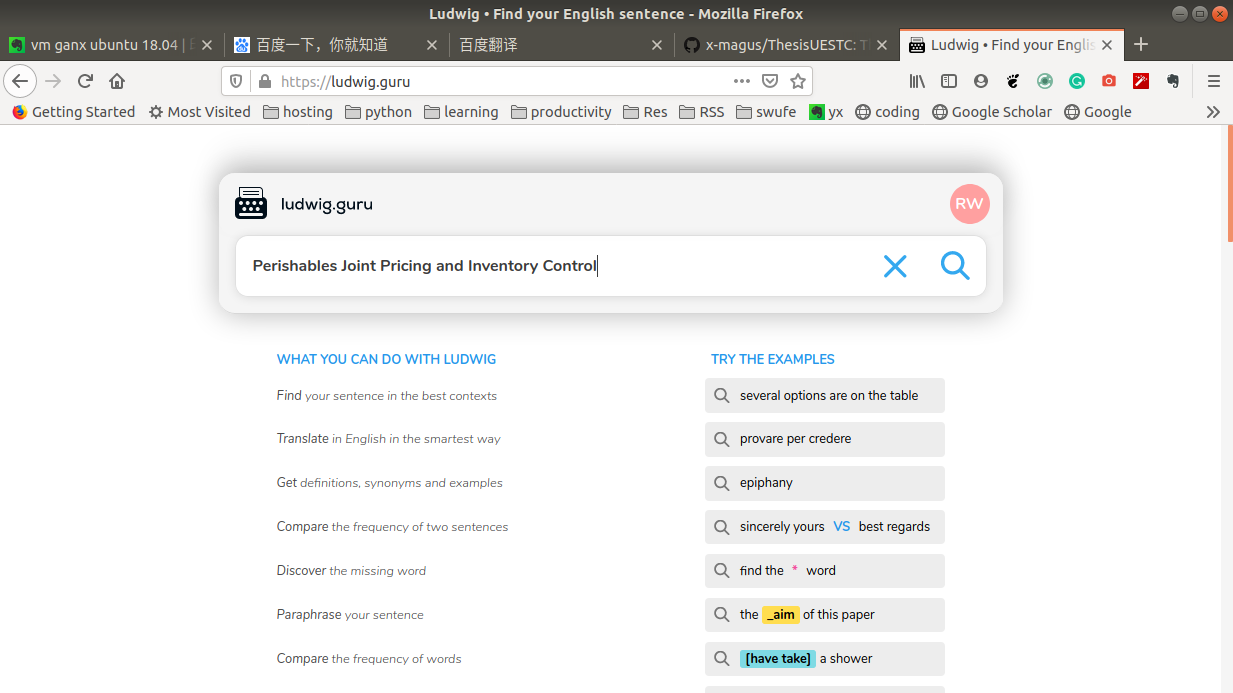
\includegraphics[width=1.0\textwidth]{media/shots/ludwig/Screenshot from 2019-12-23 21-13-03.png}
  \caption{搜索 Perishables Joint Pricing and Inventory Control}%
  \label{fig:ludwig-search}
\end{figure}

从图 \S\ref{fig:ludwig-result-1} 及 \S\ref{fig:ludwig-result-2}
可以看到,搜索的结果不理想。
因为 Ludwig 使用的语言资料库太大,搜索结果不理想时可以考虑缩小搜索范围。
注意到缺省情况下筛选功能是关闭了的(可以看到 filter OFF
字样),我们可以打开筛选选项,根据实际情况选择搜索范围。详情参见图
\S\ref{fig:ludwig-filter}.

令人遗憾的是,搜索结果任然不理想(见图
\S\ref{fig:ludwig-result-3}),没有看到完整的匹配,只看到左中位置显示的 60
SIMILAR 提示。
这时,我们可以考虑搜索更少的关键词。
从搜索结果中,我们发现 Perishables
和其它关键词甚少关联,可以考虑去掉这个关键词后重新搜索。
搜索结果见图 \S\ref{fig:ludwig-result-4},
我们可以看到仍然没有得到完美匹配,只看到 60 SIMILAR 提示。
但令人欣慰的是,在第一个结果中,我们看到了除大小写外的完美匹配。
可以理解成这个搜索是大小写敏感的。
这时我们可以考虑把搜索框中的大写字母全部改成小写字母来搜索。
搜索结果见图 \S\ref{fig:ludwig-result-5}, 我们可以看到两个完美匹配
(2 EXACT).

\begin{figure}[!htbp]
  \centering
  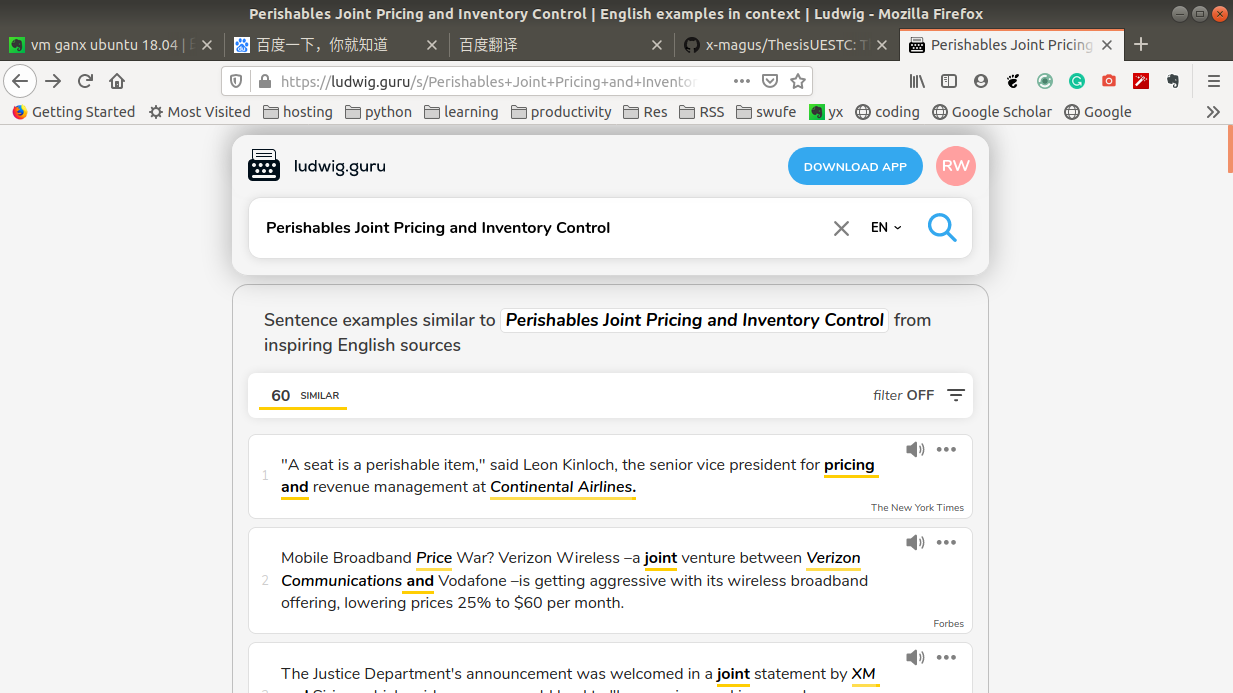
\includegraphics[width=1.0\textwidth]{media/shots/ludwig/Screenshot from 2019-12-23 21-16-43.png}
  \caption{搜索结果 1}%
  \label{fig:ludwig-result-1}
\end{figure}

\begin{figure}[!htbp]
  \centering
  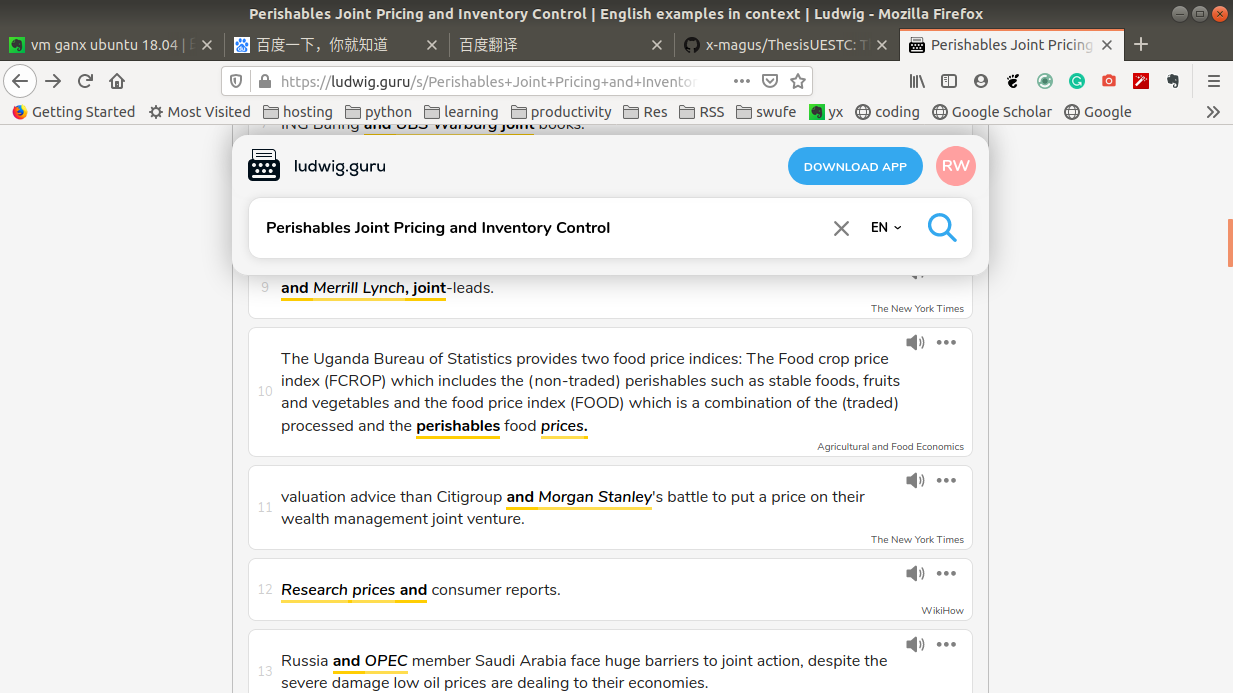
\includegraphics[width=1.0\textwidth]{media/shots/ludwig/Screenshot from 2019-12-23 21-16-55.png}
  \caption{搜索结果 2}%
  \label{fig:ludwig-result-2}
\end{figure}

\begin{figure}[!htbp]
  \centering
  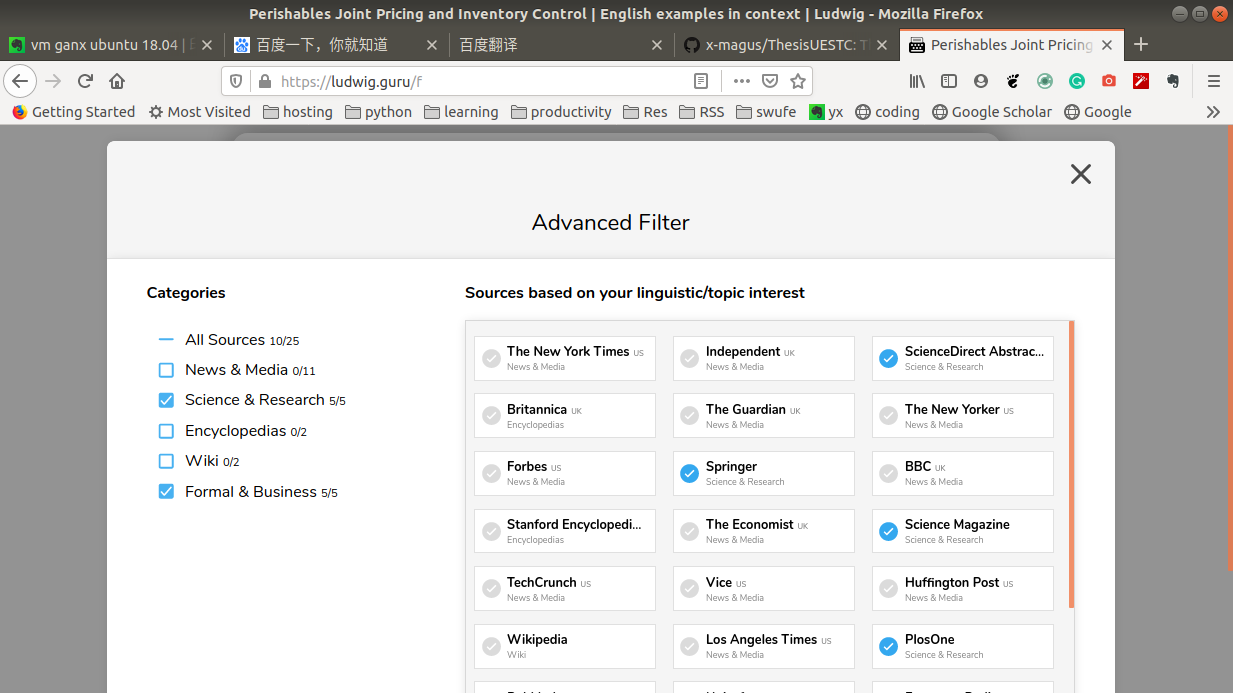
\includegraphics[width=1.0\textwidth]{media/shots/ludwig/Screenshot from 2019-12-23 21-17-32.png}
  \caption{筛选搜索范围}%
  \label{fig:ludwig-filter}
\end{figure}

\begin{figure}[!htbp]
  \centering
  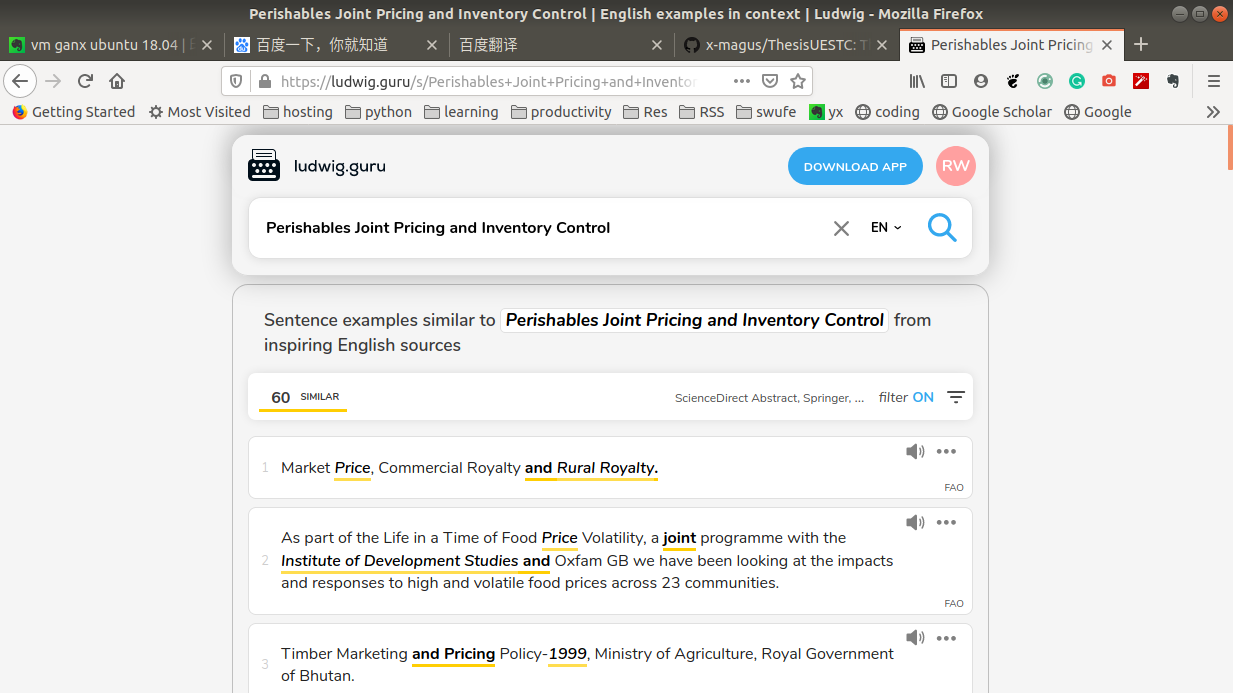
\includegraphics[width=1.0\textwidth]{media/shots/ludwig/Screenshot from 2019-12-23 21-18-09.png}
  \caption{搜索结果 3}%
  \label{fig:ludwig-result-3}
\end{figure}

\begin{figure}[!htbp]
  \centering
  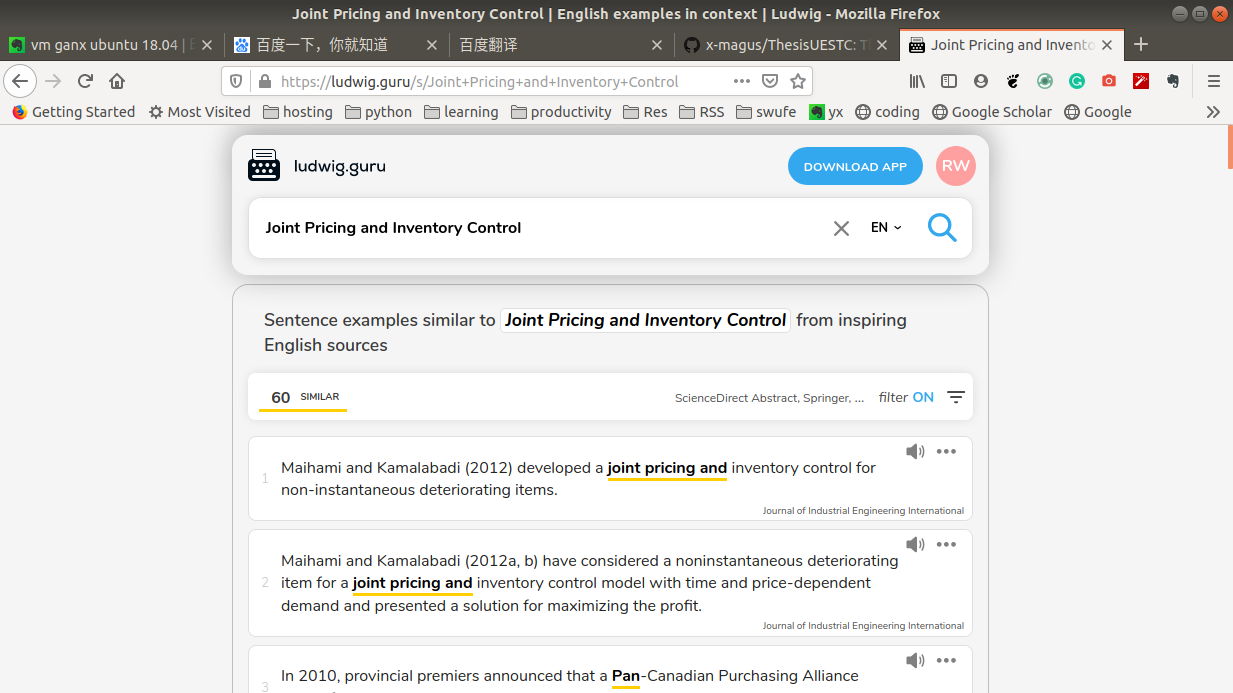
\includegraphics[width=1.0\textwidth]{media/shots/ludwig/Screenshot from 2019-12-23 21-19-22.png}
  \caption{去掉 Perashables 后的搜索结果}%
  \label{fig:ludwig-result-4}
\end{figure}

\begin{figure}[!htbp]
  \centering
  \includegraphics[width=1.0\textwidth]{media/shots/ludwig/Screenshot from
  2019-12-23 21-20-01.png}
  \caption{去掉 Perashables 后且使用小写字母的搜索结果}%
  \label{fig:ludwig-result-5}
\end{figure}



%\nocite{*}

%\bibliography{reference}

\appendix

\chapter{系统设置}%
\label{cha:settings-system-appendix}

\section{VirtualBox 虚拟机}%
\label{sec:vbox-appendix}

\subsection{故障排除}%
\label{sub:vim-troubleshooting}

\subsubsection{gVim 打开文件后不见光标}%
\label{ssub:vim-ts-cursor}

\begin{enumerate}
    \item 最大化虚拟机窗口(参见
        \S\ref{ssub:vbox-set-window-size})后打开文件,
        若能见光标就停止,否则进入下一步。
    \item 打开 \lstinline{~/.gvimrc_customized}, 修改
        \lstinline{linespace} 的设置。比如,可以尝试  \lstinline{0 - 4}
        之间的一个值。
\end{enumerate}

\subsection{图解操作}%
\label{sub:vbox-graphic-illustration}

\subsubsection{设定共享目录的图示}%
\label{ssub:vbox-set-share-folder-a}

\begin{figure}[!htbp]
  \centering
  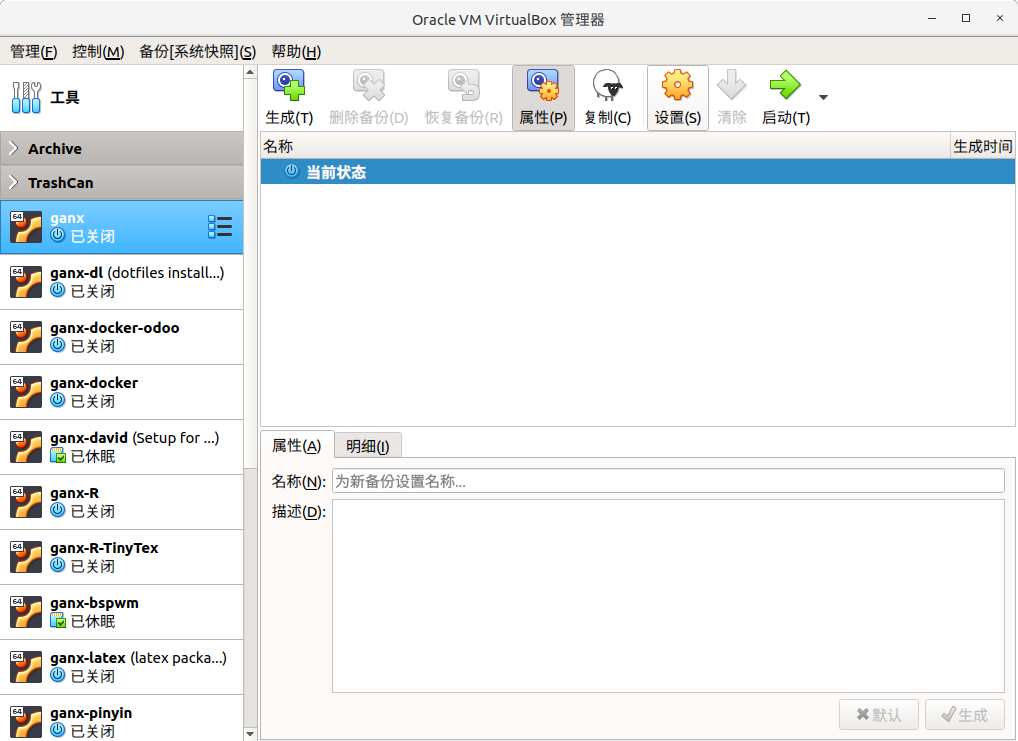
\includegraphics[width=0.9\textwidth]{media/shots/vm/Screenshot from 2019-11-29 17-52-45.png}
  \caption{设定共享目录 --- 示意图 1}
\end{figure}
\begin{figure}[!htbp]
  \centering
  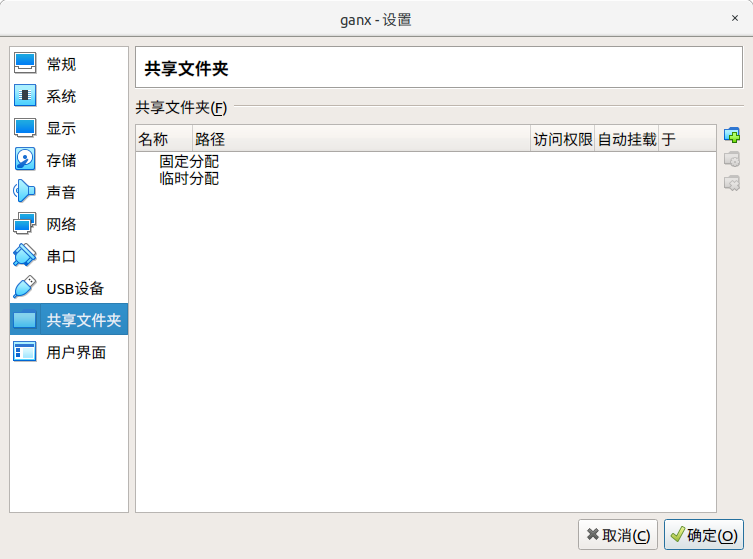
\includegraphics[width=0.9\textwidth]{media/shots/vm/Screenshot from 2019-11-29 17-53-28.png}
  \caption{设定共享目录 --- 示意图 2}
\end{figure}
\begin{figure}[!htbp]
  \centering
  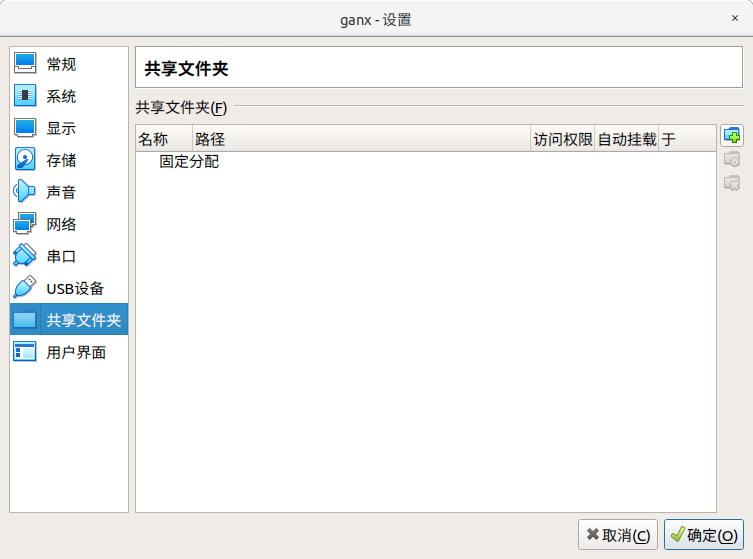
\includegraphics[width=0.9\textwidth]{media/shots/vm/Screenshot from 2019-11-29 17-54-41.png}
  \caption{设定共享目录 --- 示意图 3}
\end{figure}
\begin{figure}[!htbp]
  \centering
  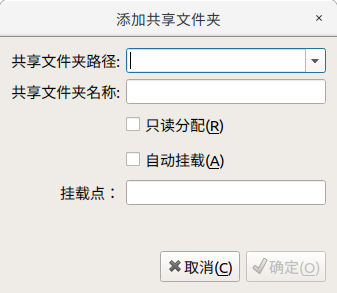
\includegraphics[width=0.9\textwidth]{media/shots/vm/Screenshot from 2019-11-29 17-55-59.png}
  \caption{设定共享目录 --- 示意图 4}
\end{figure}
\begin{figure}[!htbp]
  \centering
  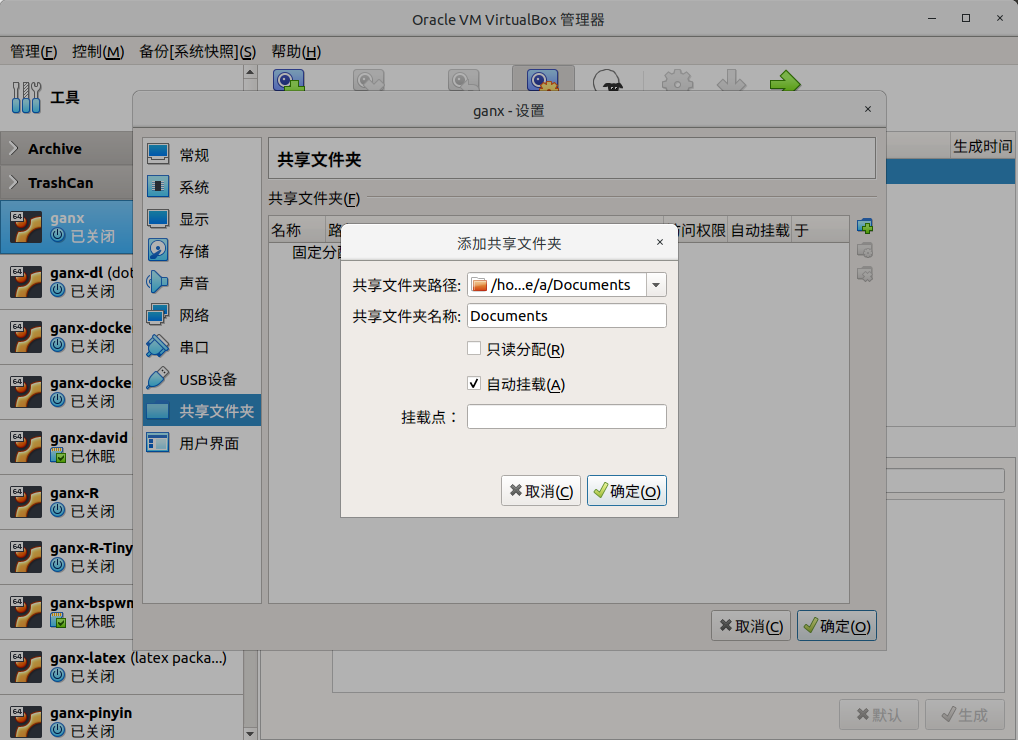
\includegraphics[width=0.9\textwidth]{media/shots/vm/Screenshot from 2019-11-29 17-59-22.png}
  \caption{设定共享目录 --- 示意图 5}
\end{figure}

\section{Linux 系统}%
\label{sec:linux-a}

\subsection{Linux 参考资料}%
\label{sub:linux-refs}

\begin{itemize}
    \item 官方网址: \href{https://www.linux.org/}{https://www.linux.org/}
    \item Ubuntu~~: \href{https://cn.ubuntu.com/}{https://cn.ubuntu.com/}
    \item 社区讨论:
        \href{https://forum.ubuntu.com.cn/}{https://forum.ubuntu.com.cn/}
    \item 问答网站:
        \href{https://askubuntu.com/}{https://askubuntu.com/}
    \item Linux 教程:
        \begin{itemize}
            \item \lstinline{Ubuntu desktop help}\footnote{
                按 \lstinline{F1} 即可以打开。}
            \item \href{https://help.ubuntu.com/lts/ubuntu-help/index.html}
                {Ubuntu 桌面指南}
            \item \href{https://linuxtools-rst.readthedocs.io/zh_CN/latest/}
                {Linux 工具快速教程}
            \item \href{https://dunwu.github.io/linux-tutorial/#/}
                {Linux 教程}
        \end{itemize}
\end{itemize}

% \subsection{Linux 基本知识}%
% \label{sub:linux-intro}


\subsection{Linux 点文件~(dotfiles)配置}%
\label{sub:dotfiles-settings}

\subsubsection{点文件介绍}%
\label{ssub:dotfiles-settings-intro}

在 Unix/Linux/Mac 系统上,软件有它们各自的配置文件,通常以~. 开头,
管它们叫 \emph{点文件}~(~\texttt{dotfiles}).
这些点文件数量多,并且所在的位置还有所不同,管理起来并不是一个容易的事情。
一个方法是把所有的这些配置文件放进一个文件夹,对每个配置文件用命令
\lstinline{ln -s} 链接到原来的位置。
这个文件夹可以用 git 仓库进行管理,
可以方便我们把一台电脑上的配置,同步到另外的电脑上。

作者配置的虚拟机上使用
\href{https://github.com/anishathalye/dotbot}{dotbot} 技术来管理 dotfiles.
在本虚拟机的 \lstinline{~/.df/} 目录中有两个文件夹: \lstinline{dotfiles}
中的配置文件是所有电脑中都共同拥有的; \lstinline{dotfiles-local}
中的配置文件是某个电脑所特有的。
建议本教程的读者在未掌握 \lstinline{dotfiles}
的配置前,不要更改这两个文件夹中的任何文件。
% \begin{tip}\label{note:vim-customized}
%     如果要对 Vim 做一些个性化的设置,可以参考 \S\ref{ssub:vim-config}.
% \end{tip}

%\subsubsection{使用本虚拟机的注意事项}%
%\label{ssub:vbox-guest-ganx}

\subsubsection{同步点文件的 Git 仓库}%
\label{ssub:vbox-guest-ganx-conf}

本虚拟机的配置文件主要由以下两个仓库控制:
\begin{itemize}
    \item \href{https://github.com/sierxue/dotfiles}
        {https://github.com/sierxue/dotfiles}
    \item \href{https://github.com/sierxue/dotfiles-local}
        {https://github.com/sierxue/dotfiles-local}
\end{itemize}

\subsubsection{设置点文件仓库的更新提示}%
\label{ssub:vbox-guest-ganx-conf-update-notification}

两个仓库不时更新的,更新配置文件的提交实现后,会发出更新提示。
如果你 \lstinline{watch (关注)} 了这两个仓库,就可以收到更新提示。
设置步骤如下:
\begin{enumerate}
    \item 访问 \href{https://github.com/sierxue/dotfiles}
        {https://github.com/sierxue/dotfiles}, 点击右上方
        \lstinline{watch (关注)} 旁边的下拉菜单,选择 \lstinline{watching}.
        如果你觉得这个仓库还有用的话,顺便点一下右边的 \lstinline{star}.
    \item 访问 \href{https://github.com/sierxue/dotfiles-local}
        {https://github.com/sierxue/dotfiles-local},
        点击右上方 \lstinline{watch (关注)} 旁边的下拉菜单,
        选择 \lstinline{watching}.
        如果你觉得这个仓库还有用的话,顺便点一下右边的 \lstinline{star}.
    \item 访问 \href{https://github.com/settings/notifications}
        {https://github.com/settings/notifications},
        配置你接收提示的选项。缺省设置下,你会在电子邮件里收到你关注的仓库的
        提交。你还可以打钩 \lstinline{Web and Mobile} 选项。
\end{enumerate}

\subsubsection{更新点文件 --- 手动方式}%
\label{ssub:update-dotfiles-manual}

\begin{enumerate}
    \item 运行下面几个命令,更新 \href{https://github.com/sierxue/dotfiles}
        {https://github.com/sierxue/dotfiles}:
\begin{lstlisting}[style=lst]
cd ~/.df/dotfiles
git checkout .
git pull --rebase
git submodule update --remote --recursive
./install
\end{lstlisting}
    \item 运行下面几个命令,更新
        \href{https://github.com/sierxue/dotfiles-local}
        {https://github.com/sierxue/dotfiles-local}:
\begin{lstlisting}[style=lst]
cd ~/.df/dotfiles-local
git checkout .
git pull --rebase
git submodule update --remote --recursive
./install
\end{lstlisting}
\end{enumerate}

\subsubsection{更新点文件 --- 自动方式}%
\label{ssub:update-dotfiles-crontab}

\begin{enumerate}
    \item 本虚拟机已经将~\S\ref{ssub:update-dotfiles-manual}~中的所有命令写入
\begin{lstlisting}[style=lst]
~/.df/dotfiles-local/scripts/pullDotfiles.sh
\end{lstlisting}
        脚本 \lstinline{pullDotfiles.sh} 的内容见 Github
        \href{https://github.com/sierxue/scripts/blob/master/pullDotfiles.sh}
        {链接}。
    \item 运行命令 \lstinline{crontab -l}, 确认你看到以下内容:
\begin{lstlisting}[style=lst]
SHELL=/usr/bin/zsh
PATH=/sbin:/bin:/usr/sbin:/usr/bin
MAILTO=""

@hourly  /usr/bin/zsh ~/.df/dotfiles-local/scripts/pullDotfiles.sh >> ~/.df/log/pullDotfiles.log
\end{lstlisting}
\end{enumerate}

\subsection{安装和设置基于 Ubuntu 18.04 的虚拟机}%
\label{sub:vbox-vm-u18-install-set}

\subsubsection{虚拟机基本信息}%
\label{ssub:linux-ubuntu}

\begin{table}[H]
   \centering
     \begin{tabular}{llllll}
     \toprule
     系统 & 初始安装 & 用户名 & 密码 & 登录方式 \\
     \midrule
     Ubuntu 18.04 & 最小安装 & ganx   & 9 & 自动登录\\
     \bottomrule
     \end{tabular}%
   \label{tab:theorem-class}%
\end{table}%

\subsubsection{设置 keyring 的密码为空}%
\label{ssub:vm-keyring}

做此设置以及初始安装时设置的 ``自动登录''后,
可以不输入任何密码使用虚拟机。
% next

\subsubsection{设置 sudo 时不询问密码}%
\label{ssub:vm-sudo}
\begin{enumerate}
    \item \lstinline{sudo gedit /etc/sudoers.d/ganx}
    \item 写入下面两行:
\begin{lstlisting}[style=lst]
User_Alias      NORMAL = ganx
NORMAL  ALL = NOPASSWD: ALL
\end{lstlisting}
    \item \lstinline{sudo chmod 0440 /etc/sudoers.d/ganx}
\end{enumerate}

\subsubsection{切换软件源}%
\label{ssub:vm-source}
% next

\subsubsection{映射 CapsLock 键到 Ctrl 键}%
\label{ssub:vm-caps-ctrl}

CapsLock 键的位置非常好,但因为 Unix 用户经常要用 Ctrl 键而从来不用 CapsLock,
所以做此映射。
% next

\subsubsection{安装虚拟机的 Guest Additions}%
\label{ssub:vbox-guest-additions}
\begin{itemize}
    \item \textbf{Windows 系统}:参考
        \href{https://www.virtualbox.org/manual/UserManual.html#additions-windows}{官方使用手册}
        安装 \lstinline{Guest additions}.
    \item \textbf{Mac 系统}: \textbf{不需要}~安装
        \lstinline{Guest additions}.
    \item \textbf{Linux 系统}: 参考
        \href{https://www.virtualbox.org/manual/UserManual.html#additions-linux}{官方使用手册}
    \item \textbf{Linux 系统 Debian 系列}:
        \begin{enumerate}
            \item \lstinline{sudo apt update}
            \item \lstinline{sudo apt install build-essential gcc make perl dkms menu}
            \item \lstinline{mount} 安装盘
                \lstinline{VBoxGuestAdditions.iso},~%
                在光盘目录下运行如下命令安装:
                 \begin{center}\label{center:vm-guest-additions}
                     \lstinline{sh ~./VBoxLinuxAdditions.run}
                 \end{center}
        \end{enumerate}
\end{itemize}
\begin{note}\label{note:ubuntu-update}
    用 \lstinline{sudo apt install} 安装任何软件之前,都需要运行
    \lstinline{sudo apt install} 来确保软件源提供的软件是最新的。
    在教程的余下部分,我们省略掉这条命令以节省篇幅。
\end{note}

\subsubsection{授予用户创建共享目录的权限}%
\label{ssub:vbox-ganx-vboxsf}
\lstinline{sudo usermod -a -G vboxsf ganx}

\subsubsection{安装设置工具 tweak}%
\label{ssub:vm-treak}

% next

\subsubsection{安装 i-bus 拼音}%
\label{ssub:pinyin-i-bus}
\begin{enumerate}
    \item \lstinline{sudo apt install ibus-libpinyin pinyin-database}
    \item 安装中文语言。
    \item 将 ``intelligent pinyin'' 加入 ``Input source''.
\end{enumerate}

\subsubsection{安装搜狗拼音}%
\label{ssub:pinyin-sogou}
\begin{enumerate}
    \item 在 \href{https://pinyin.sogou.com/linux/}
        {https://pinyin.sogou.com/linux/} 下载 64 位版本的安装包。\footnote{
            安装本虚拟机时下载的版本是
            \lstinline{sogoupinyin_2.3.1.0112_amd64.deb}
        }
    \item \lstinline{sudo apt -y install fcitx fcitx-bin fcitx-table-all}
    \item \lstinline{sudo dpkg -i sogoupinyin_2.3.1.0112_amd64.deb}
    \item \lstinline{sudo apt-get install -f}
    \item 在系统设置中的语言设置选择缺省输入方式为 fcitx.
\end{enumerate}

\subsubsection{安装配置终端 zsh}%
\label{ssub:vm-zsh}

\begin{lstlisting}[style=lst]
sudo apt install curl zsh zsh-doc
sh -c "$(curl -fsSL https://raw.github.com/robbyrussell/oh-my-zsh/master/tools/install.sh)"
chsh -s $(which zsh)
\end{lstlisting}

\subsubsection{安装版本控制软件 Git}%
\label{ssub:vm-git}

\begin{lstlisting}[style=lst]
sudo apt install git gitk git-gui
\end{lstlisting}

\subsubsection{安装编辑软件 Vim}%
\label{ssub:vm-apt-vim}

\begin{lstlisting}[style=lst]
sudo apt install vim vim-common vim-gnome
\end{lstlisting}

\subsubsection{安装 pdf 阅读软件 zathura}%
\label{ssub:vm-zathura}

\begin{lstlisting}[style=lst]
sudo apt install zathura
sudo apt install xdotool
\end{lstlisting}

\subsubsection{安装文献管理器 zotero}%
\label{ssub:vm-zotero}

在 \href{https://www.zotero.org/download/}{www.zotero.org/download/}
下载安装包 \lstinline{Zotero-5.x.xx_linux-x86_64.tar.bz2}.
然后运行如下命令:
\begin{lstlisting}[style=lst]
sudo tar -xf ~/Documents/tools/Zotero-.x.xx_linux-x86_64.tar.bz2 -C /opt
sudo bash /opt/Zotero_linux-x86_64/set_launcher_icon
sudo ln -s /opt/Zotero_linux-x86_64/zotero.desktop /usr/share/applications/
sudo chown -R ganx: /opt/Zotero_linux-x86_64
\end{lstlisting}



\printindex
\printglossary[title={术语表}]

\end{document}
